\documentclass[10pt,times]{beamer}
\usepackage{amsfonts}
\usepackage{amsmath}
\usepackage{amssymb}
\usepackage{mathptmx}

\usepackage{color}
\usepackage{minted}
\usepackage{hyperref}
\usepackage{multicol}
\usepackage{multirow}
\usepackage{tabularx}
\usepackage{booktabs}
\usepackage{menukeys}
\usepackage{subcaption}

% ******************************** Meta-data ***********************************
\mode<presentation>
{
  \usetheme{Madrid}
  \setbeamercovered{transparent}
}


\usepackage{caption}
\captionsetup{font=scriptsize, labelfont=scriptsize, justification=centering}

\title{An introduction to heterogenous computing}

\author {Krishna Kumar \inst{*}\thanks{github.com/kks32} }

\institute[ University of Cambridge ] % (optional, but mostly needed)
{
%  \includegraphics[width=0.9\textwidth]{figs/goto.png}
}

%\pgfdeclareimage[height=0.2cm]{uni}{figs/Engineering.png}
% \logo{\pgfuseimage{uni}}

\date[\today]{\today}
% Delete this, if you do not want the table of contents to pop up at
% the beginning of each subsection:
\AtBeginSection[]
{
  \begin{frame}<beamer>{Outline}
    \tableofcontents[currentsection,currentsubsection]
  \end{frame}
}


% If you wish to uncover everything in a step-wise fashion, uncomment
% the following command: 

%\beamerdefaultoverlayspecification{<+->}

\subtitle{Accelerating numerical codes}
%***************************** Title page **************************************
\begin{document}
\begin{frame}
  \titlepage
\end{frame}

%*******************************************************************************
%******************************* Frame *****************************************
%*******************************************************************************
\section{Overview: Architecture}

\begin{frame}{von Neumann Architecture}
\begin{columns}
\column{.6\linewidth}
\begin{itemize}
\item Hungarian mathematician John von Neumann circa~1940 - the general 
requirements 
for an electronic computer.
\item ``Stored-program computer" - both program instructions and data are 
kept in 
electronic memory.
\begin{itemize}
\item \textit{Read/write}, random access memory is used to store both 
program 
instructions and data.

\item \textit{Control unit} fetches instructions/data from memory, decodes 
the 
instructions and then sequentially coordinates operations to accomplish the 
programmed task.

\item \textit{Aritmetic Unit} performs basic arithmetic operations

\item \textit{Input/Output} is the interface to the human operator 
\end{itemize}

\end{itemize} 

\column{.495\linewidth}
\begin{figure}
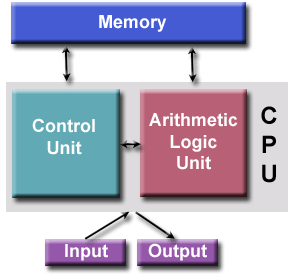
\includegraphics[width=0.7\linewidth]{figs/vonNeumann}
\caption*{Basic architecture}
\end{figure}
\end{columns}
\end{frame}


%*******************************************************************************
%******************************* Frame 
%*****************************************
%*******************************************************************************

\begin{frame}{Serial computing}

\begin{itemize}
\item Traditionally, software has been written for serial computation:
\begin{itemize}
\item A problem is broken into a discrete series of instructions
\item Instructions are executed sequentially one after another
\item Executed on a single processor
\item Only one instruction may execute at any moment in time 
\end{itemize}

\end{itemize} 

\begin{figure}
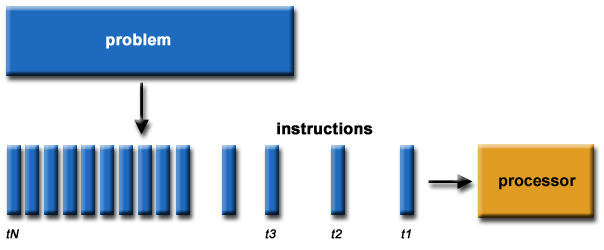
\includegraphics[width=0.7\linewidth]{figs/serial}
\caption*{}
\end{figure}
\end{frame}


%*******************************************************************************
%******************************* Frame 
%*****************************************
%*******************************************************************************

\begin{frame}{Memory model}
\begin{columns}
\column{0.49\textwidth}
\begin{figure}
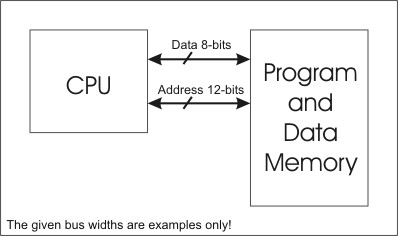
\includegraphics[width=.7\linewidth]{figs/ideal_memory_model}
\caption*{Ideal memory model: \\ We write for this architecture}
\end{figure}

\column{0.49\textwidth}
\begin{figure}
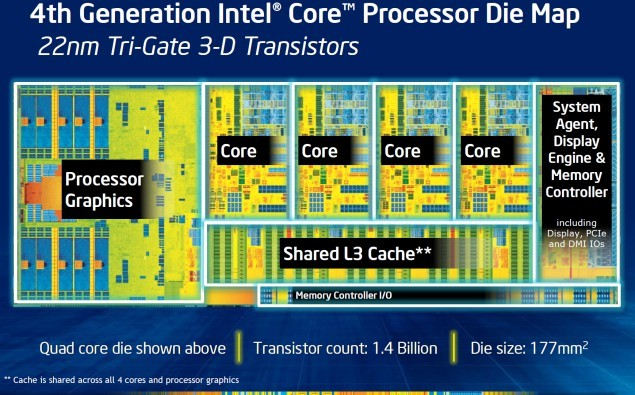
\includegraphics[width=0.9\linewidth]{figs/real_memory_model}
\caption*{Real memory model: How it actually looks}
\end{figure}
\end{columns}

\centering
\textit{The underlying assumption is cache coherency!}
\flushleft
\small
In a shared memory multiprocessor with a separate cache memory for each 
processor, it is possible to have many copies of any one instruction 
operand: one 
copy in the main memory and one in each cache memory. When one copy of an 
operand is 
changed, the other copies of the operand must be changed also. Cache 
coherency 
ensures that changes in the values of shared operands are propagated 
throughout the 
system in a timely fashion.
\end{frame}


%*******************************************************************************
%******************************* Frame 
%*****************************************
%*******************************************************************************
\begin{frame}{What are caches}
\begin{columns}
\column{0.49\textwidth}
\begin{figure}
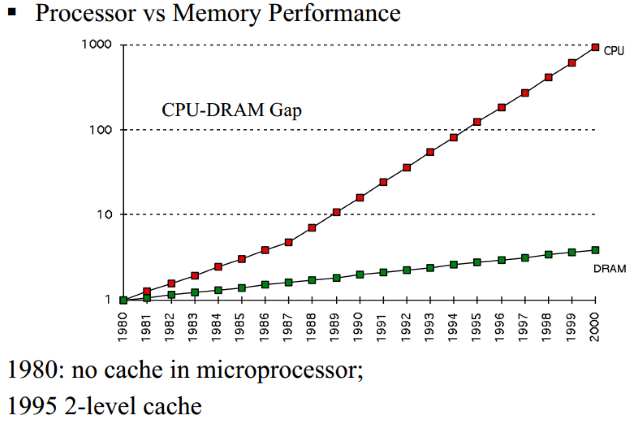
\includegraphics[width=0.9\linewidth]{figs/CPU_DRAM}
\caption*{CPU vs DRAM}
\end{figure}

\column{0.49\textwidth}
\begin{figure}
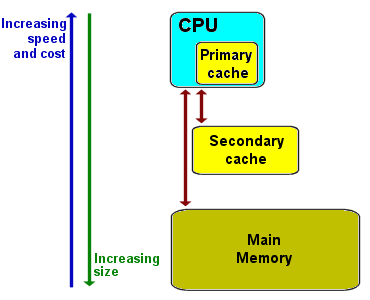
\includegraphics[width=.7\linewidth]{figs/cache}
\caption*{Cache}
\end{figure}
\end{columns}
\begin{itemize}
\item CPU caches are small pools of memory that store information the CPU 
is most 
likely to need next.

\item A cache miss means the CPU has to go scampering off to find the 
data elsewhere. This is where the L2 cache comes into play — while it's 
slower, it's 
also much larger. 

\item If data can't be found in the L2 cache, the CPU continues down the 
chain to L3 
(typically still on-die), then L4 (if it exists) and main memory (DRAM).

\end{itemize}
\end{frame}


%*******************************************************************************
%******************************* Frame 
%*****************************************
%*******************************************************************************
\begin{frame}{Does your compiler execute the program you wrote?}

\begin{quotation}
\textbf{No, absolutely not! Compiler most often says ``you didn't intend to 
write 
that. I have a better idea...''}
\end{quotation}
\begin{itemize}
\item \textit{Sequential consistency:} Executing the program you wrote.

``the result of any execution is the same as if the operations of all the
processors were executed in some sequential order, and the operations of
each individual processor appear in this sequence in the order specified
by its program.'' - Lesslie Lamport

\item \textit{Compiler optimisation}
\item \textit{Processor execution}
\item \textit{Cache coherency}
\item Chip / compiler design annoyingly helpful:
\begin{itemize}
\item It can be expensive to exactly execute what you wrote
\item Often they rather do something else, that's faster
\end{itemize}
\end{itemize}
\end{frame}


%*******************************************************************************
%******************************* Frame 
%*****************************************
%*******************************************************************************
\begin{frame}[fragile]{Does your compiler execute the program you wrote?}
\begin{columns}
\column{0.5\textwidth}

\begin{minted}[mathescape, linenos,
               numbersep=5pt,
               gobble=0,
               frame=lines,
               framesep=2mm]{c++}
// Your code
for (i = 0; i < rows; ++i) {
  for (j = 0; j < cols; ++j) {
    a[j*rows+i]+=42;
  }
}
\end{minted}

\column{0.5\textwidth}
\begin{minted}[mathescape, linenos,
               numbersep=5pt,
               gobble=0,
               frame=lines, obeytabs=true, showtabs=true,
               framesep=2mm]{c++}
// Compiler optimised version
for (j = 0; j < cols; ++j) {
  for (i = 0; i < rows; ++i) {
    a[j*rows+i]+=42;
  }
}
\end{minted}
\end{columns}
\vskip3em
The CPU will expect a sequential operation. Iterating through each row of 
data is faster than going through each column. Almost always, a 2D matrix 
is stored as a 1D linear array.
\end{frame}


\end{document}